\documentclass{standalone}
\usepackage{pgfplots}
\pgfplotsset{compat=1.7}

\begin{document}
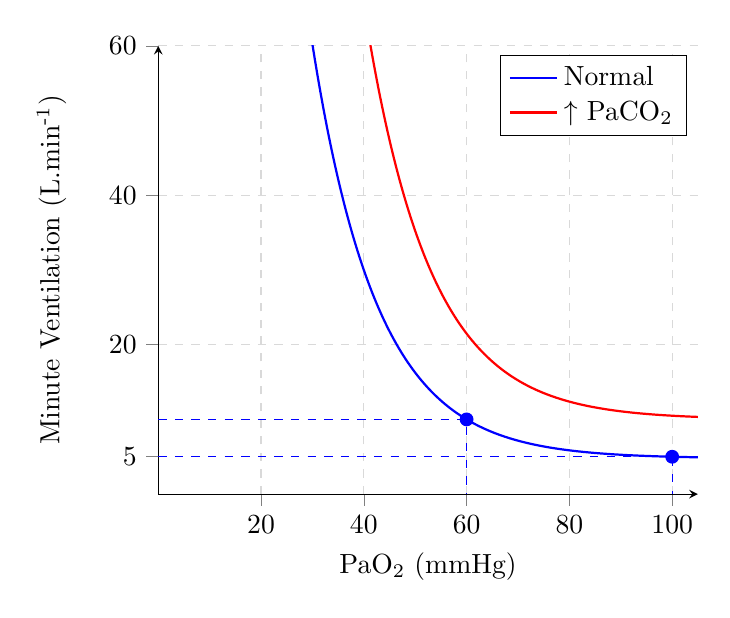
\begin{tikzpicture}
    \begin{axis}[
        axis x line=middle,
        axis y line=middle,
        grid = major,
        grid style={dashed, gray!30},
    	  x label style={at={(axis description cs:0.5,-0.1)},anchor=north},
	  y label style={at={(axis description cs:-0.1,.5)},rotate=90,anchor=south},
	extra y ticks={5},
extra y tick labels = {5},
        xmin=0,
        xmax= 105,
        ymin= 0,
        ymax= 60,
	 ylabel near ticks,
	xlabel near ticks,
        xlabel=PaO\textsubscript{2} (mmHg),
        ylabel=Minute Ventilation (L.min\textsuperscript{-1}),
        tick align=outside,
        enlargelimits=false,
legend cell align={left}]
	\coordinate (o) (0,0);
	\addplot[domain=20:105, blue, thick,samples=500] {4.775923 + 588.0668*e^(-0.07872604*x)};
\addlegendentry{Normal}
	\draw [thin, blue, dashed] (axis cs: 0,10) -- (axis cs: 60,10) node[circle,fill=blue,inner sep=0pt,minimum size=5pt]{} -- (axis cs: 60,0);
	\draw [thin, blue, dashed] (axis cs: 0,5) -- (axis cs: 100,5) node[circle,fill=blue,inner sep=0pt,minimum size=5pt]{} -- (axis cs: 100,0);
	\addplot[domain=20:105, red, thick,samples=500] {10 + 588.0668*e^(-0.07872604*(x-10))};
\addlegendentry{$\uparrow$ PaCO\textsubscript{2}};

\end{axis}

\end{tikzpicture} 
\end{document}